% 
%jff-notes
%
\documentclass[11pt]{article}
\usepackage[pdftex]{graphicx}
\usepackage{amssymb}
\usepackage{latexsym}
%\usepackage{relsize}
\usepackage{textcomp}
%processed for 10 pt 
%\documentstyle[epsf,psfig]{article}
%\documentstyle[epsf]{article}
\oddsidemargin 0pt
\topmargin -0.0cm
\textwidth 6.2in
\textheight 8.5in
\baselineskip 18pt
%\renewcommand{\baselinestretch} {1.5}
\newenvironment{nitemize}
   {\begin{list}{\begin{math}\bullet\end{math}}%
      {\setlength{\leftmargin}{5mm}
       \setlength{\topsep}{1mm}
       \setlength{\parsep}{0in}
       \setlength{\itemsep}{.7mm}}}%
   {\end{list}}

\newcommand{\fract}[2]{\frac{\textstyle #1}{\textstyle #2}}
\newcommand{\trans}[3]{#1 \stackrel{#2}{\longrightarrow} #3}
\newcommand{\notrans}[3]{#1 \stackrel{#2}{\not\! \longrightarrow} #3}
\bibliographystyle{plain}
\begin{document}
\title{A simple CW plugin for SDRuno (Version 3)}
\author{
Jan van Katwijk\\
Lazy Chair Computing \\
The Netherlands\\
{\em J.vanKatwijk@gmail.com}}
%\date{}
\maketitle
%\baselineskip 22pt
\ \\
\ \\
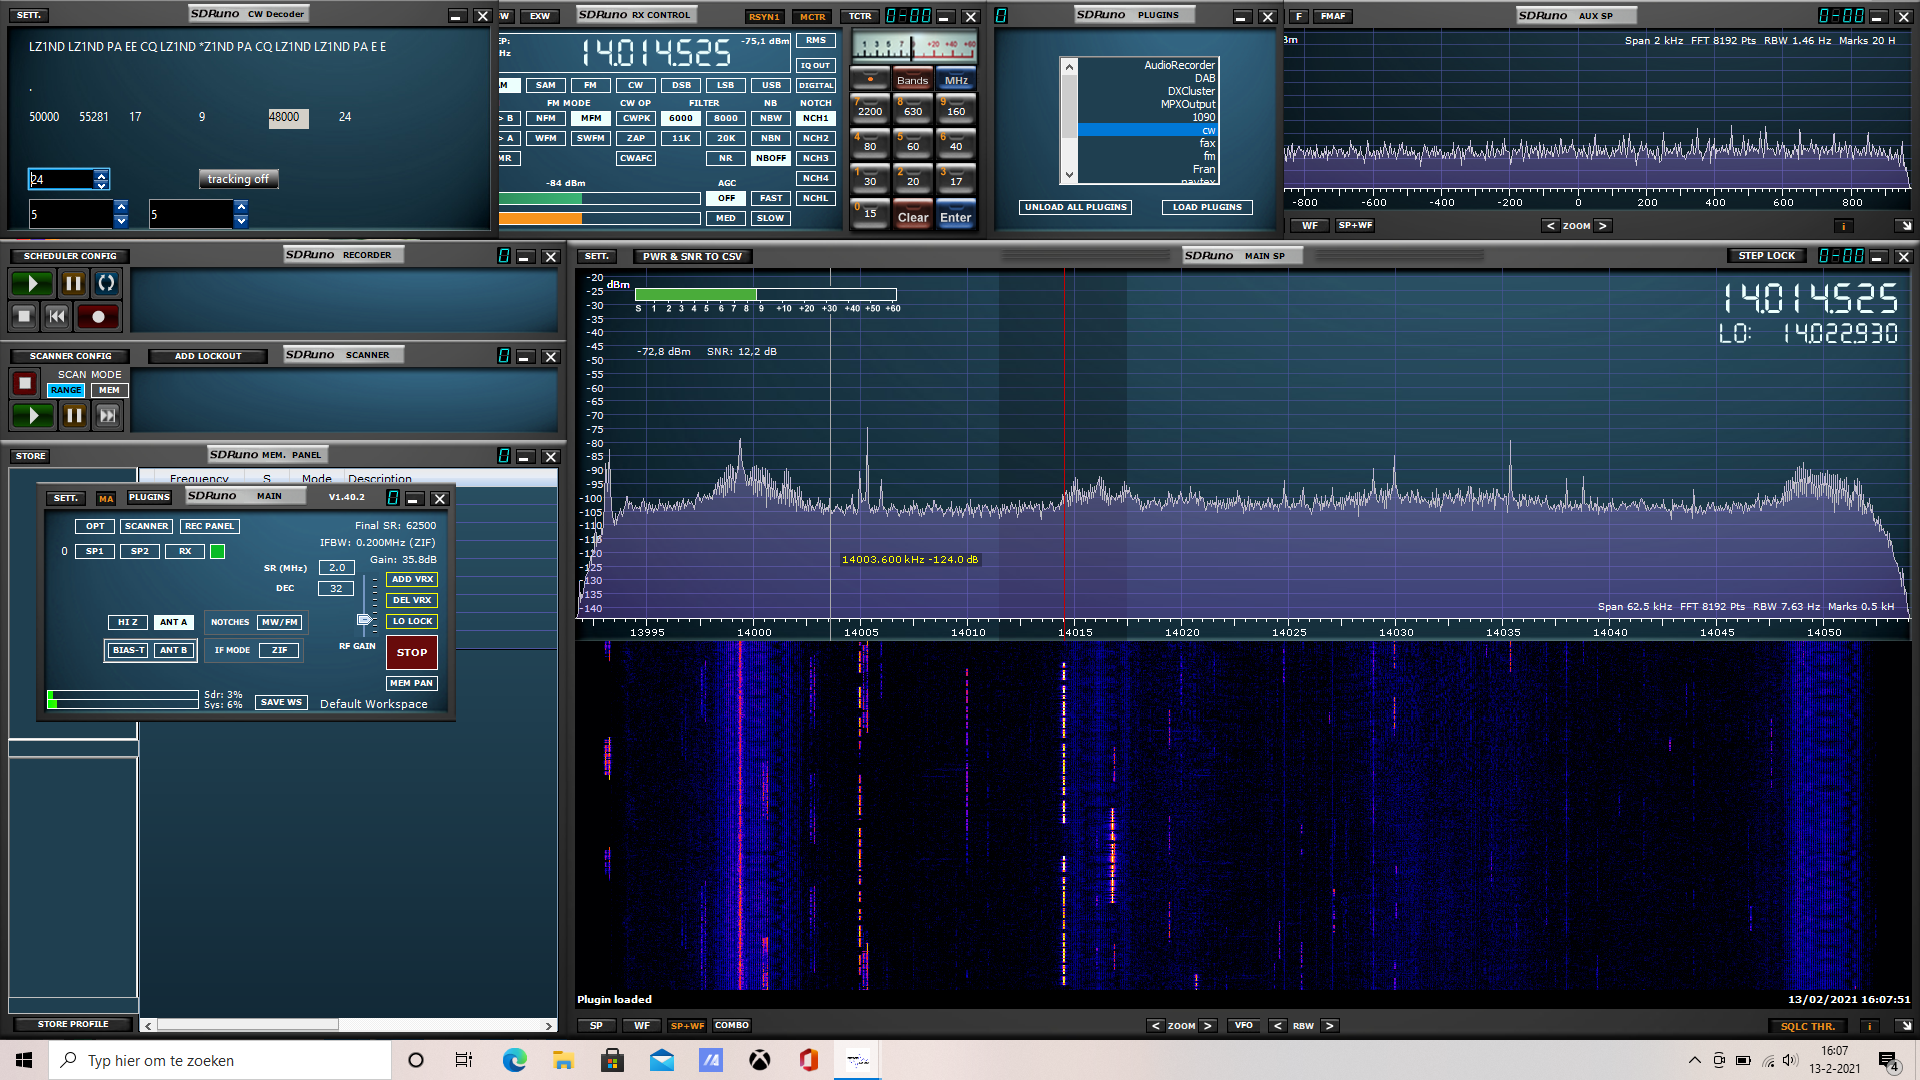
\includegraphics[width=140mm]{cw-example.png}
\ \\
\section{Introduction}
The SDRuno cw plugin is a simple plugin to decode CW (Continuous Waves) signals.
CW is in amateur bands still very popular, I am usually looking at the
14 MHz band. 

\section{Settings}
CW (basically carrier on/carrier off) is a signal with a small footprint,
the width used on  the band can be less than 50 Hz.
The decoder therefore works with an intermediate
samplerate of 2000 samples/second.
\par
This implementation select the so-called {\em IQ-OUT} option, so
decosing basically uses the unprocessed input, down-sampled to 192000.
One should realize that the SDRuno spectrum display shows default a
wide band, the advantage is that one sees a lot of signals, the disadvantage
is that precise tuning, based on the view on the spectrum is not easy.

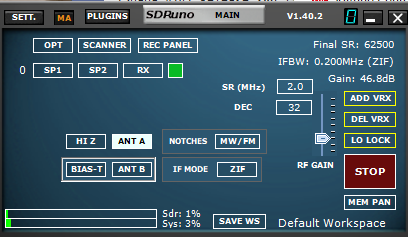
\includegraphics[width=100mm]{main-widget.png}

The plugin generates an audiotone of 800 Hz + the tuning offset,
At least for me, some sound helps with tuning.

\section{Tuning}
As said, CW is a signal with a small footprint, and since many of
the amateur transmissions are brief messages (such as CQ CQ ...), tuning
requires some training.
\par
What is really helpful is {\em zooming in} on the main display.
\includegraphics[width=100mm]{main-spectrum-display.png}

To ais in tuning, this version of the decoder is equipped with
an automatic tuning aid.
{\em Within a (user specified) range, the plugin will tune to the strongest signal,}

\section{The plugin}
The plugin widget  is shown in the picture

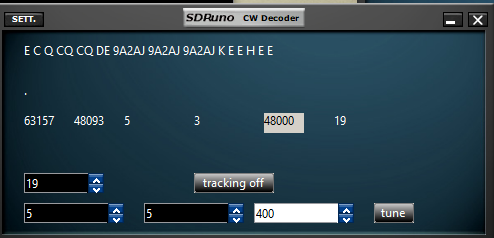
\includegraphics[width=100mm]{cw-plugin-widget.png}

The main issue with CW decoding is that different operators use different
transmission speeds.
The way the plugin works is that the {\em duration} of the signal above
a certain noise level is measured. As known, a dot and a space within the
encoding of a letter have the same length, while a dash is supposed to take 3 times as much time.
Experience shows that most operators transmit with app 25 to 30 words per
minute. The spinbox - in the picture set to "19" - can be used to adapt 
the wpm estimate.

The top line in the widget shows the received text,
the second line - in the picture only containing a single dot -
displays the dots and dashes of the letter currently being received.
The third line contains 6 number displays, from left to right
\begin{itemize}
\item the number of micro seconds {\em assumed} as duration for a dot. The 
number is computed by looking at the setting for the words per minute;
\item the number of micro seconds {\em measured} as (average) duration of
the spaces between dots and dashes;
\item the strength of the signal;
\item the strength of the noise floor;
\item the audio output rate; 
\item the current words per minute setting.
\end{itemize}

As said, the next row contains a selector for the assumed words per minute.
It furthermore contains a button labeled {\em tracking off}. If a transmission
is seen with a duration longer than a few seconds, a tracker can be activated
that adapts the assumed WPM. However, for transmissions of 3, 4 seconds
as usually seen on the 14 MHz band, it is not advisable to set the tracker on.

The number display in this row tells the computed offset/ 

Finally, the bottom row contains three spinboxes and a button:
\begin{itemize}
\item the {\em filter depth}. Before attempting to decode the on/off appearance
of the carrier, a lowpass filter is applied to the signal. The actual
degree of the (FIR) filter is twice the amount on the selector plus 1.
\item the {\em squelch level}. To distinguish signal from noise, a squelch level
can be set.
\item the width of the fine tuning search. The picture shows "400", indicating
that - with the current frequency as middle - a segment of 400 Hz is searched
for the strongest signal if "fine tuning" is on.
\item the button, when touched will reset the automatic tuning aid.
\end{itemize}
\end{document}

